\section*{Stories - Splitting - Why?}
Are you splitting a story to fit into an iteration? This is splitting a story for an arbitrary reason. You can make your stories bigger or smaller by lengthening or shortening your iteration.

Here are some better reasons for splitting stories:
\begin{itemize}
\item A story can be split to make it less complex.
\item A story can be split to deliver the most important features first.
\item A story can be split to allow for emergent design.
\end{itemize}

\clearpage
\section*{Stories - Splitting - Incremental Features - 1}
\subsection*{Setup}
\begin{figure}[ht]
\centering
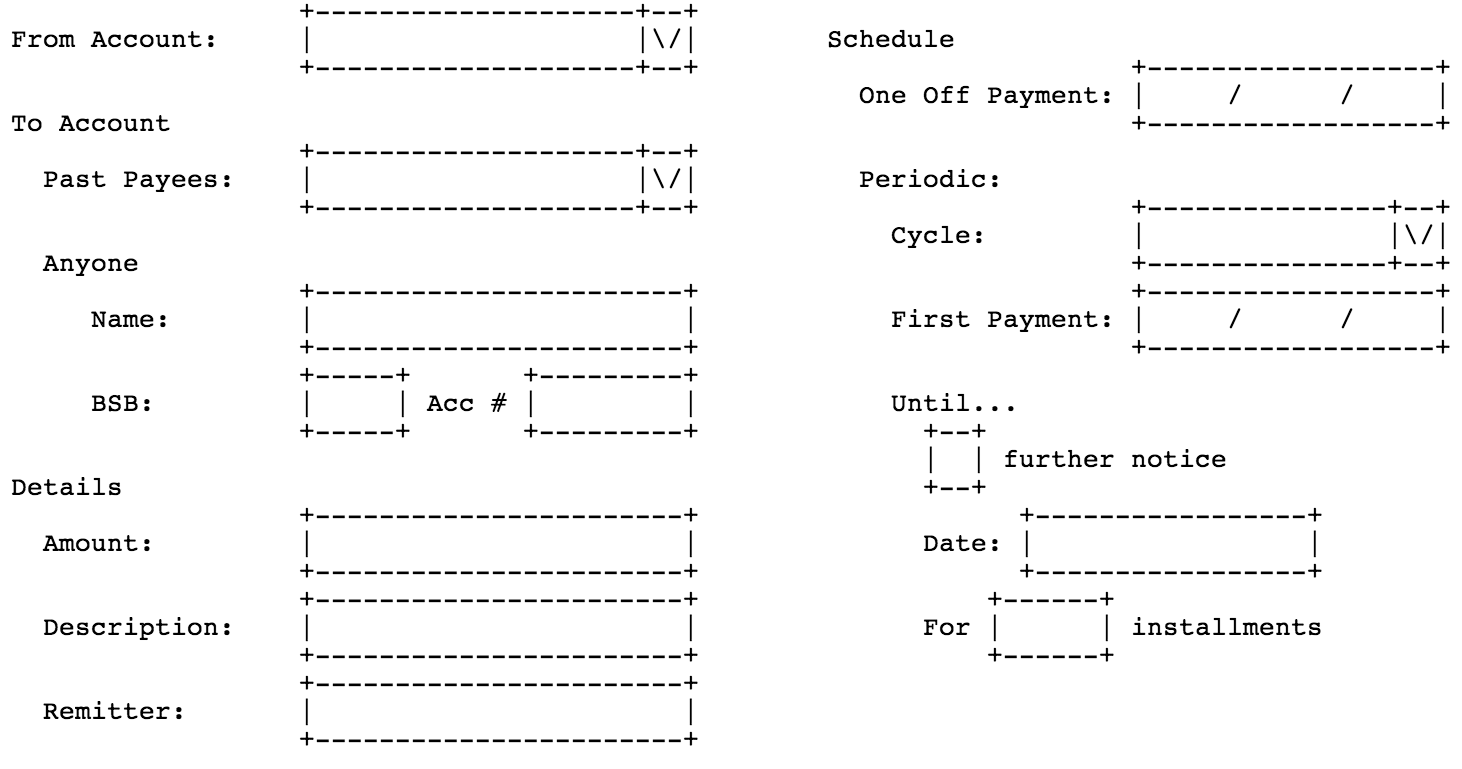
\includegraphics[scale=0.3]{stories/banking_wireframe.png}
\caption{Draw on the whiteboard the following online banking site. This is the end state or what the customer wants.}
\end{figure}


\clearpage
\section*{Stories - Splitting - Incremental Features - 2}
\subsection*{Setup}
Enumerate the features on the board:
\begin{itemize}
\item pay anyone
\item one off payment
\item future payment
\item recurring payment open ended
\item recurring payment future dated
\item recurring payment end dated
\item pay previous payee
\end{itemize}

\section*{Stories - Splitting - Incremental Features - 3}
\subsection*{the exercise}
The group has to suggest how they would split the work and which piece of work they would do first.

\subsection*{notes}
\begin{itemize}
\item The one off payment to anyone is the easiest thing to do
\item Redirect discussions of splitting the work based on "make the UI but have the buttons not work" back to a useful discussion about delivering incremental functionality.
\end{itemize}

\clearpage
\section*{Stories - Splitting - Acceptance Criteria}
Flesh out the acceptance criteria for a story, and this is based on 'separation of concerns' approach to splitting criteria.

Could the story go without one or two criterion? If so, could these be cleaved off into their own story?

\clearpage
\section*{Stories - Splitting - Technical Complexity - 1}
This technique allows for both the fostering of new ideas as well as the identification of the first story with the least amount of effort. In our example we are going to plan for a 'Mobile Offline Wikipedia' application.

The required functionality is:
\begin{itemize}
\item download the data onto the device
\item building an index for searching
\item searching and search results
\item formatting of a wiki page
\item marking a page as a favourite
\end{itemize}

\clearpage
\section*{Stories - Splitting - Technical Complexity - 2}
Draw on the whiteboard a five by five grid of boxes like so:

\begin{tabular*}{0.75\textwidth}{@{\extracolsep{\fill} } c | c | c | c | c | }
 no frills &  & initial &  & bells \& whistles \\
  \hline                        
  & & download data & & \\
    \hline                        
  & & indexing & & \\
    \hline                        
  & & search \& results & & \\
    \hline                        
  & & page display & & \\
    \hline                        
  & & favourites & & \\
  \hline  
\end{tabular*}

Muddy the waters by mentioning that downloading data needs to consider failed downloads, the 4GB limit on android operating systems, updates and slow connections. The search results need to handle no results found, one result and pagination. Result display needs to handle the plethora of device resolutions in existence.

\clearpage
\section*{Stories - Splitting - Technical Complexity - 3}
Ask the group to suggest how they could do it differently. Put each answer in a box. Simpler solutions go on the no frills side and fancy features and exciting uses of technology go on the bells \& whistles side.

\subsection*{Example}
\begin{tabular}{ c | c | c | c | c | }
 no frills &  & initial &  & bells \& whistles \\
  \hline                        
  copy from PC & basic download & ... & restart failures & auto-sync \\
    \hline                        
   alphabetic & subject index & ... & tailored index & \\
    \hline                        
  exact match & partial match & ... & autocomplete & search suggestion\\
  & & & fuzzy match & voice recognition \\
    \hline                        
  plain text  & portrait only & ... & font size & many resolutions\\ 
  & & & custom styles &  \\
    \hline                        
  none & & ... & sync'd favs & \\
  \hline  
\end{tabular}

\clearpage
\section*{Stories - Splitting - Technical Complexity - 4}
You will see that most groups are very good at adding exciting new features on. Once they have filled up that side of the board suggest that their are simpler solutions out there if they think about it. The exercise isn't over until the left-most column is populated.

Once complete you can then show the team that the first story they should play is the left most column. This is the MVP that will provide all the functionality requested and prove the system. Once complete and feedback has been received the product owner can then cherry pick features off the grid as single stories. Autocomplete is a single story. As is partial matching.

A team will need to do this exercise for each feature they want to implement.